\documentclass{report}

\usepackage{titlesec}
\usepackage{titling}
\usepackage{hyperref}
\usepackage[margin=1in]{geometry}
\usepackage[normalem]{ulem}
\usepackage[dvipsnames]{xcolor}
\usepackage{graphicx}
\usepackage[framemethod=TikZ]{mdframed}
\usepackage{etoolbox}
\usepackage{listings}
\usepackage{indentfirst}

% sets up mdframed
\newcounter{defi}[section]\setcounter{defi}{0}
\renewcommand{\thedefi}{\arabic{section}.\arabic{defi}}
\newenvironment{defi}[2][]{%
\refstepcounter{defi}%
\ifstrempty{#1}%
{\mdfsetup{%
frametitle={%
\tikz[baseline=(current bounding box.east),outer sep=0pt]
\node[anchor=east,rectangle,fill=blue!20]
{\strut Definition~\thedefi};}}
}%
{\mdfsetup{%
frametitle={%
\tikz[baseline=(current bounding box.east),outer sep=0pt]
\node[anchor=east,rectangle,fill=blue!20]
{\strut Definition~\thedefi:~#1};}}%
}%
\mdfsetup{innertopmargin=10pt,linecolor=blue!20,%
linewidth=2pt,topline=true,%
frametitleaboveskip=\dimexpr-\ht\strutbox\relax
}
\begin{mdframed}[]\relax % Added this line
}{%
\end{mdframed} % Added this line
}

% Example usage of mdframed
% \begin{defi}[Pythagoras' theorem]{defi:pythagoras}
% In a right triangle, the square of the hypotenuse is equal to the sum of the squares % of the catheti.
% $$a^2+b^2=c^2$$
% \end{defi}

% setup listings for code blocks
% -- colors
% Define a custom color
\usepackage{color}
\definecolor{darkred}{rgb}{0.6,0.0,0.0}
\definecolor{darkgreen}{rgb}{0,0.50,0}
\definecolor{lightblue}{rgb}{0.0,0.42,0.91}
\definecolor{orange}{rgb}{0.99,0.48,0.13}
\definecolor{grass}{rgb}{0.18,0.80,0.18}
\definecolor{pink}{rgb}{0.97,0.15,0.45}

%custom style:
\lstset{
  aboveskip=1em,
  breaklines=true,
  abovecaptionskip=-6pt,
  captionpos=b,
  escapeinside={\%*}{*)},
  frame=single,
  numbers=left,
  numbersep=15pt,
  numberstyle=\tiny,
}
% 0. Basic Color Theme
\lstdefinestyle{colored}{ %
  basicstyle=\ttfamily,
  backgroundcolor=\color{white},
  commentstyle=\color{green}\itshape,
  keywordstyle=\color{blue}\bfseries\itshape,
  stringstyle=\color{red},
}
% 1. General Python Keywords List
\lstdefinelanguage{PythonPlus}[]{Python}{
  morekeywords=[1]{,as,assert,nonlocal,with,yield,self,True,False,None,} % Python builtin
  morekeywords=[2]{,__init__,__add__,__mul__,__div__,__sub__,__call__,__getitem__,__setitem__,__eq__,__ne__,__nonzero__,__rmul__,__radd__,__repr__,__str__,__get__,__truediv__,__pow__,__name__,__future__,__all__,}, % magic methods
  morekeywords=[3]{,object,type,isinstance,copy,deepcopy,zip,enumerate,reversed,list,set,len,dict,tuple,range,xrange,append,execfile,real,imag,reduce,str,repr,}, % common functions
  morekeywords=[4]{,Exception,NameError,IndexError,SyntaxError,TypeError,ValueError,OverflowError,ZeroDivisionError,}, % errors
  morekeywords=[5]{,ode,fsolve,sqrt,exp,sin,cos,arctan,arctan2,arccos,pi, array,norm,solve,dot,arange,isscalar,max,sum,flatten,shape,reshape,find,any,all,abs,plot,linspace,legend,quad,polyval,polyfit,hstack,concatenate,vstack,column_stack,empty,zeros,ones,rand,vander,grid,pcolor,eig,eigs,eigvals,svd,qr,tan,det,logspace,roll,min,mean,cumsum,cumprod,diff,vectorize,lstsq,cla,eye,xlabel,ylabel,squeeze,}, % numpy / math
}
% 2. New Language based on Python
\lstdefinelanguage{PyBrIM}[]{PythonPlus}{
  emph={d,E,a,Fc28,Fy,Fu,D,des,supplier,Material,Rectangle,PyElmt},
}
% 3. Extended theme
\lstdefinestyle{colorEX}{
  basicstyle=\ttfamily,
  backgroundcolor=\color{white},
  commentstyle=\color{darkgreen}\slshape,
  keywordstyle=\color{blue}\bfseries\itshape,
  keywordstyle=[2]\color{blue}\bfseries,
  keywordstyle=[3]\color{grass},
  keywordstyle=[4]\color{red},
  keywordstyle=[5]\color{orange},
  stringstyle=\color{darkred},
  emphstyle=\color{pink}\underbar,
}


%define "squiggly" to make red squiggly underline
\makeatletter
\def\squiggly{\bgroup \markoverwith{\textcolor{red}{\lower3.5\p@\hbox{\sixly \char58}}}\ULon}
\makeatother


% Stuff to edit.
\title{CPU-Scheduling}
\newcommand{\thesubtitle}{The Illusion of Multitasking}
\newcommand{\currentdate}{2024/25}
\author{Mark Krutzler}
\newcommand{\auinstitution}{Kantonschule Im Lee}

\titleformat{\section}
{\huge\bfseries}
{\thesection}
{0.5em}
{}[\titlerule]

\titleformat{\subsection}
{\bfseries\LARGE}
{\thesection}
{0.5em}
{}

\titleformat{\subsubsection}
{\large\bfseries}
{\thesection}
{0.5em}
{}


\renewcommand{\maketitle}{
\begin{center}


{\Huge\bfseries
\thetitle}
\vspace{0.5em}\\
{\LARGE\thesubtitle}


{\rule{0.4\textwidth}{.4pt}}

{\bfseries \theauthor}\\
\textit{\auinstitution \ --- \currentdate}
\end{center}
}

\begin{document}

\begin{titlepage}
\vspace*{\fill}
\centering
\maketitle
\vspace*{\fill}
\end{titlepage}

\tableofcontents



\part{Forewords?}

\section{Introduction}


We all use computers.
The modern person couldn't do half of the things that is expected from him without an instance of Windows, MacOs or any other Operating System.
We surf the web, write emails, documents and have a video call at the same time.
The question is: "How does CPU achieve all of this?" The things listed are only the parts of the OS that we come in contact with on a daily basis.
What about all the other things hidden under the hood?
If simplified, a simple CPU is like a simple production line. It does one things at a time.
Therefore a problem arises then we have multiple tasks: The CPU can only do one thing at a time\footnote{When talking about a single-core CPU for simplification} and yet we all multitask on our machines.
This Black Box effect of taking multiple jobs and working on them in a proper order is what I will disect in this "Maturarbeit".

The art of scheduling tasks could seem easy for us humans.
We ?instinctively? estimate the many aspects of the task:
\begin{itemize}
\item Job: Convince our boss to give us a pay rise\\Priority: High\\Time Required: Medium (With a lot of waiting time)\\Effort: High (Said "No way" last week)
\item Job: Walk the Dog\\Priority: High\\Time Required: Low\\Effort: Low
\item Job: Go to the Hairdresser\\ Priority: Low (Went last week as well)\\Time Required: High\\Effort: Low
\end{itemize}
These prediction are often highly complex and are based on previous experiences.
We also include factors like: When was the last time I did it?
In addition to all that every human plans differently based on what's important to him/her.
Still from just the priority, time required and effort, we would roughly know how to order these things.
For example I would walk the dog first, because it is a "request" made by someone else and therefore the response time should be as low as possible.
The Hairdresser can fade into the background, due to its low priority. Maybe making an appointment is a good idea though.

A computer does nothing like that. How could it? What he sees is:
\begin{itemize}
\item Job: Process 1\\Priority: Needs to be Set\\Time Required: ??? (Waiting Time: ???)\\Effort: ???
\end{itemize}
What he knows is when the task arrived and how much time he worked on it.
The goal of scheduling is somehow not to rely on predictions and still decide wisely.
With this in mind the let's get to a quick introduction of the metrics, so that we know how to rate the policies that we'll look at.


\pagebreak
\section{Metrics}
% TODO: MAYBE JUST LEAVING THIS OUT AND LOOKING AT THIS DURING A LATER TIME (WHEN THE METRICS ARE MENTIONNED OR LINK AS A FOOTNOTE?)
% TODO: ALSO THIS FOLLOWS THE OSTEP WAY TOO MUCH:
We can measure different aspects of a "scheduler policy". There is however a differentiation between fairness and performance. It is often a tradeoff between the two. % TODO: Lateron mention, where it is obvious
For example the concept of everybody getting a same sized piece of cake is fair. However, it would be faster to give more to the fast eaters than to those who like to talk during eating. In this scenario we can't have both fairness and performance. In reality it is really difficult to predict, who'll eat faster.

% TODO: WAY TOO DEEP, BECAUSE WILL NEVER REALLY USE IT AGAIN THAT DEEPLY (EXCEPT IF A PROPER EXPLANATION IS DONE FOR EACH POLICY)
\begin{defi}[Turnaround Time]{dfn:turnaround}
The turnaround time is a performance metric. It measures how long a task took to be completed from the time it arrived.
It is calculated as follows:
$$T_{Turnaround} = T_{Completion} - T_{Arrival}$$
\vspace{1em}
\end{defi}

We'll often look at the Average Turnaround time for a predetermined set of jobs.
This helps us to quantify how "efficient" a single task is handeled.
In the best case scenario a single jobs turnaround time is equivalent to the runtime of that job.
Another really important thing for us is Response Time.
We want to move our mouse around.
If we type we want the letter to appear in an instant and the Microsoft suite should start without much delay.
Of course the startup time of a program depends on many other factors, however if we never even start working on it, it'll take a good while.


\begin{defi}[Response Time]{dfn:response}
The response time is a performance metric. It measures the responsiveness of our computer. How much time does it take until the job is run?
It is calculated as follows:
$$T_{Response} = T_{First\_Run} - T_{Arrival}$$
\vspace{1em}
\end{defi}



\part{The ABCs of CPU Scheduling}

\chapter{Basic Algorithms}

This chapter mainly focuses on simple policies that can be used to order processes.
Usually there are multiple simplifications added to the scenario so that it makes sense.
The policies are generally either an abstraction for though experiments or a part of a larger system.
Therefore there will be an absense of answers to common questions like: "How do we know how long a process takes until completion?" \footnote{Actually we actually never really know how long something will take}
There are also some example code snippets to each policy.
These are just so you can understand the algorithm and they don't really work in a real life scenario.
First of all they can't handle interrupts and therefore don't work in a real system.
In addition to that Python is a high level language and is absolutely not made to handle low level stuff!

\section{First In, First Out (FIFO)}

Probably the most basic of them all.
The "First In, First Our" is just as the name suggests it. 
Usually we humans know it as first come, first served. 
This policies runs into problems really quickly if we discard the possibility of all tasks requiring the same amount of run time. 
A so called "Convoy Effect" takes place. 
Just imagen how annoying it is, when you're at a store and a family of five cuts into the line in front of you. 
They have two full carts loaded. You have to wait until they finish. 
In addition to that they also send back their kid to get an extra bottle of ketchup. 
Wouldn't it be overall much faster if they let you in front before the cashier starts scanning the items?

\begin{lstlisting}[language=Python, style=colorEX, label=cd:fifo-python]
# Simple implementation of FIFO in Python
queue = []

# Adding a new process
def add_process(process):
  queue.append(process)

# Decide which process is next
def allocate():
  next = queue.pop(0)
  use_resource(next) # function that will allow "next" to use the CPU
\end{lstlisting}

As you can see the implementation is itself pretty easy.
\pagebreak

\section{Shortest Job First (SJF)}

Now the situation changes a bit. 
The infamous family of five wants to go first, however the cashier picks you after seeing that you only have a few items.
This is the "Shortest Job First" (SJF). 

\begin{lstlisting}[language=Python, style=colorEX, label=cd:sjf-python]
# Simple implementation of SJF in Python

# Define process class and queue
class Process:
  def __init__(self, burst): # burst time is the time required for the process to finish
    self.burst = burst
    # other stuff that is relevant for the process class

queue = []

# Adding a new process
process = Process(burst) 
def add_process(process): 
  queue.append(process)

# Decide which process is next
def allocate():
  queue.sort(key=lambda a: a.burst) # sort according to burst
  next = queue.pop(0)
  use_resource(next) # function that will allow "next" to use the CPU
\end{lstlisting}

There are two notable changes in this code snippet when compared to FIFO. One of them is relevant.
First, the less exiting part is that I actually took my time to write out some of the process class definition.
Second and the real difference to FIFO is that we sort the queue according to the burst time\footnote{Burst time is basically the runtime needed until the process finishes. This variable can be only predicted}. 
This means that we will choose the task with the shortest time to completion.
At this point one could go into which sort algorithm to use and which one is the most efficient, however that is not something I will touch upon here.
The reason is that I don't think that it is necessary to understand those in order to grasp the concept of SJF.

Back to our story, now you only have a problem when you arrive late. The scanning of products has already started and you'll have to wait.
This policy is a so called non-preemptive policy.
"Non-preemptive" just means that once a task will run until it finishes.


\section{Shortest Time-to-Completion First(STCF)}

If SJF and FIFO are cousins than STCF is the brother.
To fix the issue from before, we'll make SJF "preemptive", meaning that our cashier can now "save" the state of the previously scanned items. 
Therefore STCF is also called "Preemptive Shortest Job First (PSJF)".
The option of saving a state comes in handy, especially if a program has to wait for I/O.
Although the switching costs some time, this can be disregarded, because one would have to wait until the little boy returns with the ketchup\footnote{If you don't know what I am talking about read Chapter 1.1 (FIFO)} anyways.
The state of waiting is usually called "blocked" and the technique of running something else during the task is blocked is called overlapping.
% TODO: explain blocked and overlapping with the cashier in a better way
Preemptiveness also makes the computer much more responsive, because now you can really do certain things "at the same time".
The best part is that we don't even have to change much of the previous code.
\pagebreak
\begin{lstlisting}[language=Python, style=colorEX, label=cd:stcf-python]
  # Simple implementation of STCF in Python
  
  # definition of process class and queue go here
  current = Process(burst)
  current_runtime = 0
  
  # Adding a new process
  def add_process(process): 
    queue.append(process)
    allocate()
  
  # Decide which process is next
  def allocate():
    save_state() # saves of the current process

    current.burst -= current_runtime # first update burst
    current_runtime = 0

    queue.sort(key=lambda a: a.burst) # sort according to burst
    current = queue.pop(0)

    use_resource(current) # function that will allow "next" to use the CPU (also tracks runtime)
\end{lstlisting}
Whenever a new process "joins", the "allocation" function gets run.
In addition to that, whenever the process finishes, or it voluntarily gives up the CPU, the same "allocation" function can be run.


\section{Round Robin (RR)}

Now, why don't we just scan one item for everyone? 
This could mean that every one sees progress and that same sized jobs finish at almost the same time
Even if at this point the item scanning explanation doesn't really work anymore\footnote{You can't scan a fraction of a product, or can you?}, let's just make the so called "quanta" (quantum in singular) even smaller.
% TODO: Explain term quantum better
As already mentionned in the previous chapter, the cashier needs some time to "save" the state of the current purchases. 
This effectively mean that after the quantum shrinks to a certain extent, the "context switching"\footnote{Context switch saves the state of a process so that it can be restored later} would get too expensive. 
The goal is to reach a balance, where we have enough responsibility, but the price for it is not too high.
Notice how by treating the processes more "fairly" by don't caring about their overall burst time, we get rid of a variable, which can only be predicted and replace it with another one, which is more abstract and global.
\pagebreak
\begin{lstlisting}[language=Python, style=colorEX, label=cd:rr-python]
  # Simple implementation of RR in Python

  queue = []
  quantum = 1 # Adjust the time slice here

  def add_process(process):
    queue.append(process)

  def use_resource(process, quanta):
    # definition of use_resource
    # now it also takes an amount of quanta that the process can run for
    # after that it saves the state and returns.

while true:
  for process in queue:
    use_resource(process, quantum)

\end{lstlisting}

At this point it is time to advance to move onto more advanced policies.

\part{Advanced Policies}


\chapter{Multi-Level Feedback Queue}

\section{Abstract Rules}

\subsubsection{Introduction}
Here we'll look at policies that one doesn't "just invent".
These are usually more sophisticated and can be hypothetically used in a real system (at least with some adjustemts). 
First we'll look at the Multi-Level Feedback Queue, short MLFQ. 
This is one of the most known ones and is used in Solaris.
The creator Fernando J. Corbató even recieved a Turing Award for it in 1990.
First I'll write down some abstract rules. These are usually complemented with an example. 
After that there will be a quick implementation of the policy in Python.
Please feel free to jump around to get a better grasp of the (theory).

\subsubsection{Basics}

The most basic principle of MLFQ are the so called "Priority Queues". These are priorities that a program can belong into.
They can change over time and these changes reflect the action/state of a program.
The changing of the priority is done as followed: every task has a certain amount of "allotment" for each priority.
If this CPU time is used up, than the process will be moved down once and recieve a new set of allotment.
This way you could have a fast lane checkout, where you can only scan a few items.
A separation of small and bulk purchases would occur making the experience overall faster.
There is still only one cashier though, so there are some pitfall that one must avoid.

\begin{figure}[h]
  \begin{center}
    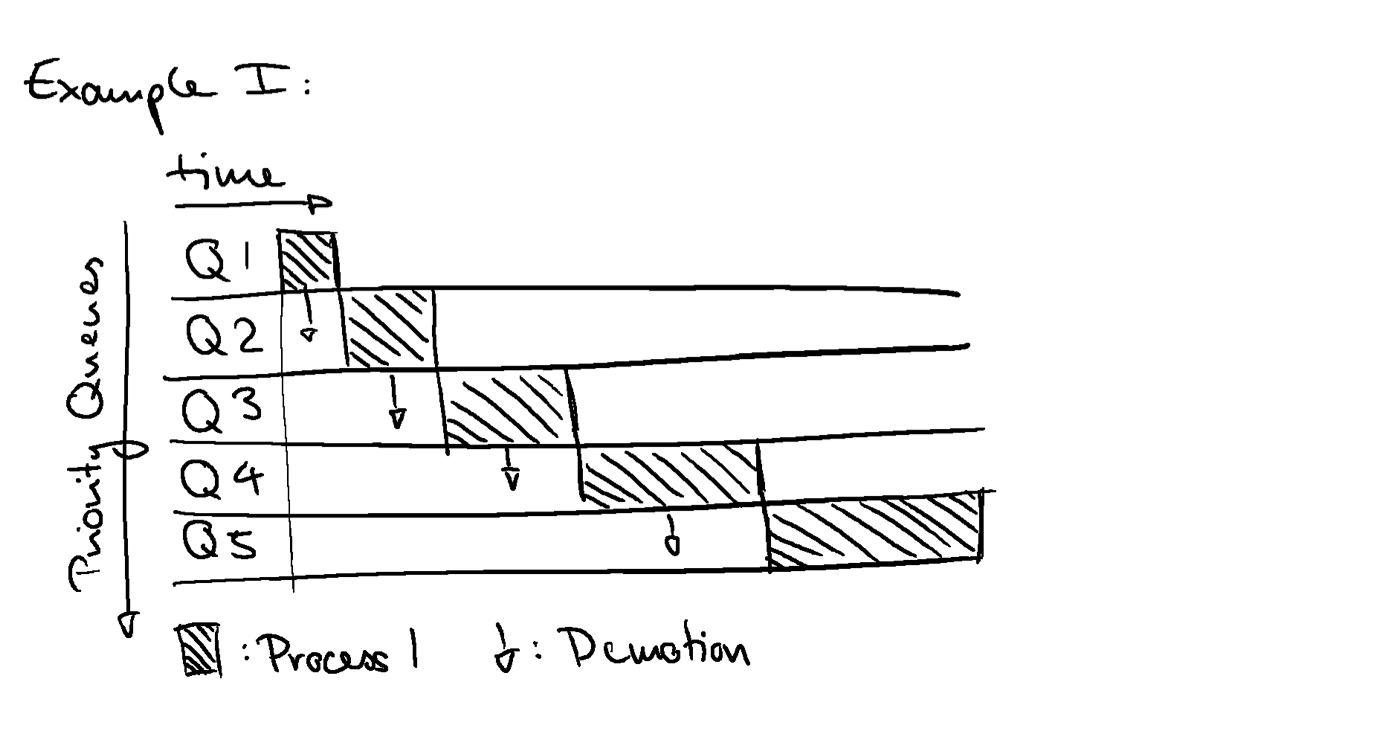
\includegraphics[width=0.7\textwidth]{assets/mlfq-diag-1.png}
    \caption{Basic Overview}
    \label{mlfq-diag-1}
  \end{center}
\end{figure}

As you can see in the figure \ref{mlfq-diag-1}, we have 5 queues. They are represented on the y axis. 
Although there are usually more than just five, too many queues would just make things more complicated. 
The x axis represents the time.
After a while process 1, gets demoted from the current queue. This happens, because it used up it's allotment.
None the less, process one keeps running, because there is no one other competing. 
However if the add another process 2, than the situation changes.

\begin{figure}[h]
  \begin{center}
    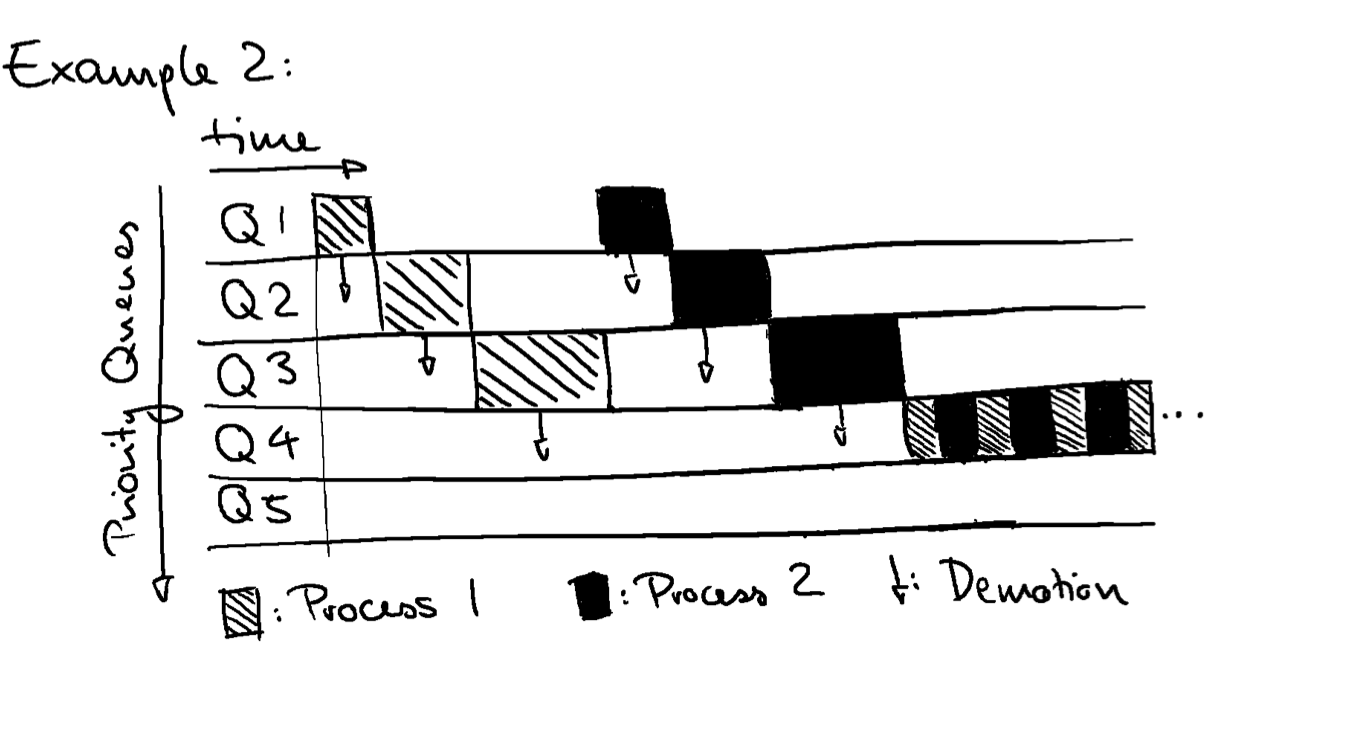
\includegraphics[width=0.7\textwidth]{assets/mlfq-diag-2.png}
    \caption{Introducing Process 2}
    \label{mlfq-diag-2}
  \end{center}
\end{figure}

As you can see processes at a higher priority are preferred over processes lower down. 
This effectively means that once process 2 joins the comptetition it can monopolize the CPU until they end up on the same level.
Once they are there Round Robin is used to give them both a fair share of allotment.
With each process starting in the highest queue, this means that the shorter tasks are generally preferred, because they can finish quickly before they end up on a lower queue. Therefore the system becomes more responsive.
Keep in mind that if a process gives up it's CPU before the allotment is used up (for example if they wait for I/O), than they will "stay" in the same priority and can use up the rest of the CPU time, before getting demoted.
% TODO: INSERT WATING TIEM EXAMPLE HERE meaning a sketch
Therefore not the actual time spent there matters, but the time spent using the resource.
As you might have to already noticed poor process 1 didn't get any runtime while process 2 was getting their priority prioperly adjusted. Note: for simplicity there are now only 4 queues.

\begin{figure}[h]
  \begin{center}
    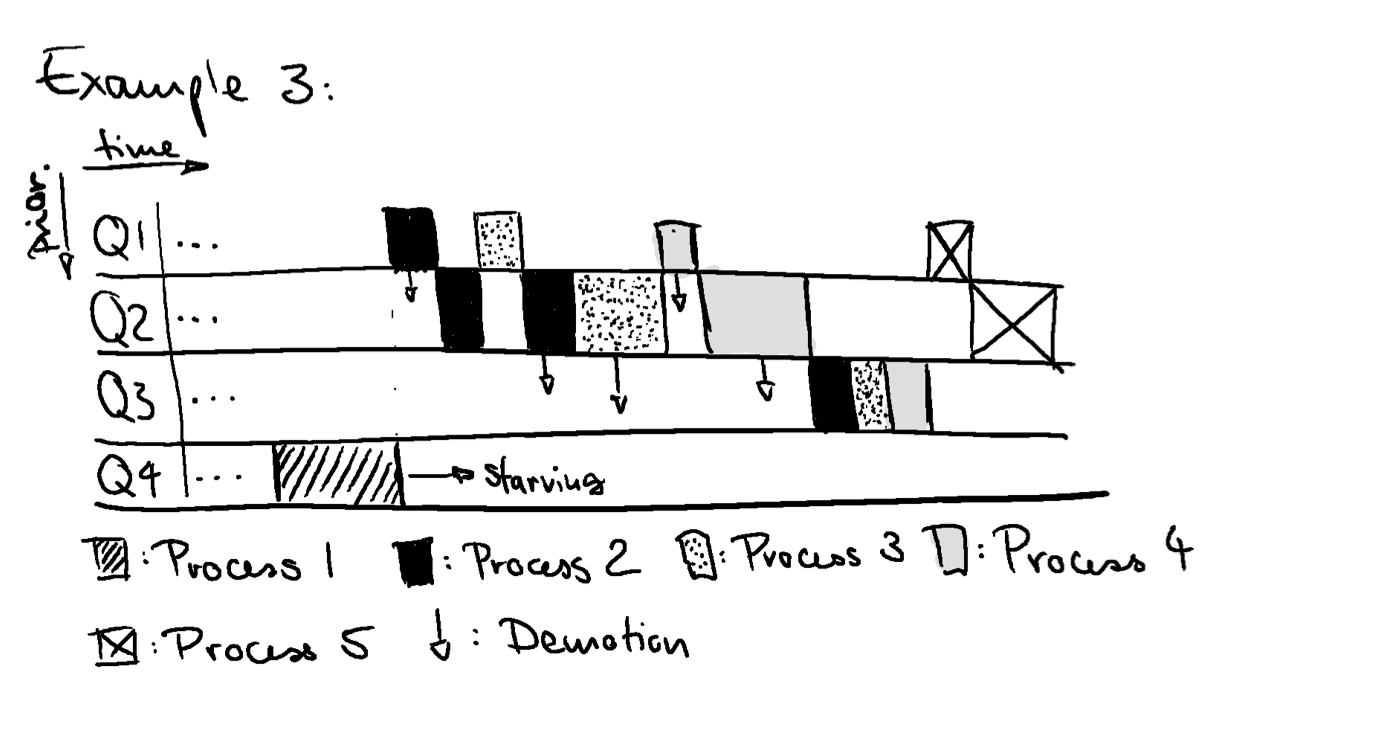
\includegraphics[width=0.7\textwidth]{assets/mlfq-diag-3.png}
    \caption{Starvation of Process 1}
    \label{mlfq-diag-3}
  \end{center}
\end{figure}

To solve the so called "starvation" issue, which essentially means that longer tasks get to the bottom priority and stay there being stuck, because there is no way to move, we'll introduce "priority boosts".
This effectively means that after a certain period S, all processes are boosted to queue 1 and therefore it gives everybody a "second chance". If the processes finish still in priority 1 or 2, than they deserved that queue.
If however the processes do not finish than they get promoted together to the bottom queue and everybody recieves a fair share.

\begin{figure}[h]
  \begin{center}
    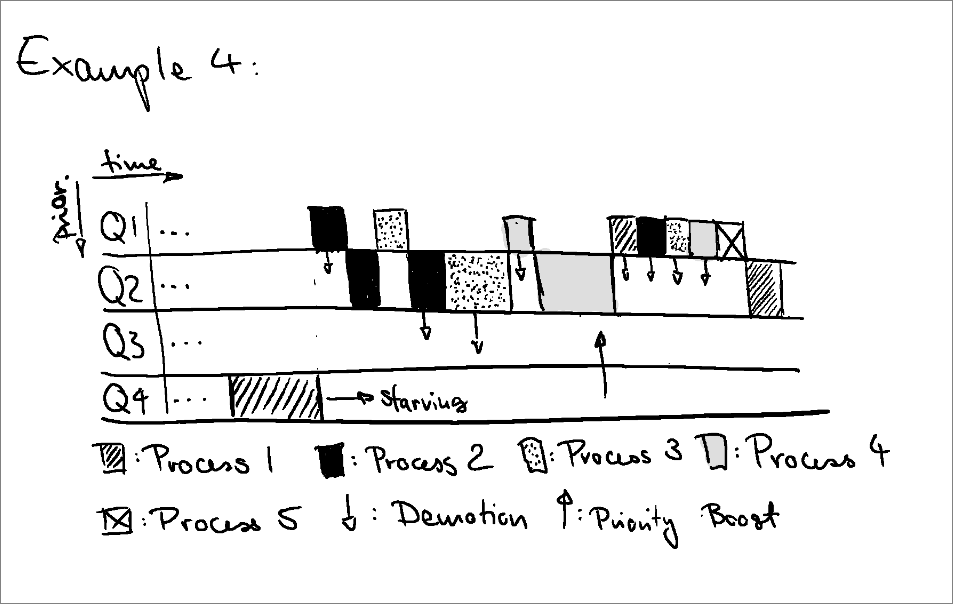
\includegraphics[width=0.7\textwidth]{assets/mlfq-diag-4.png}
    \caption{Priority Boost}
    \label{mlfq-diag-4}
  \end{center}
\end{figure}

\noindent So as "OSTEP REFERENCE HERE" would summarize it: % TODO: find and insert reference
\begin{enumerate}
  \item If Priority (A) $>$ Priority (B) $\Rightarrow$ A runs \& B doesn't
  \item If Priority (A) = Priority (B) $\Rightarrow$ A \& B run in RR
  \item When a job enters the system, it is placed at the highest priority
  \item Once a job uses up its time allotment at a given level, its priority is reduced
  \item After some period S, move all the jobs in the system to the topmost queue
\end{enumerate}

\subsubsection{Voo-Doo Constants}

Even though MLFQ introduces multiple Voo-Doo Constant, like the scheduling quantum, amount of queues, period S, allotment size (constant or changing?), % TODO: EXPALIN CONSTAND OR CHANGIN
we still gain an advantage over just simply unknown constant like the burst time or a predetermined priority and effort. These are huge improvements, because this means that we could actually implement it properly and the use case is not just purely a though experiment. 
It makes sense to find some sensible defaults for these constants and let the system admin adjust it, if they feel like it. One could find these magic numbers through machine learning, however that is out of scope of the topic?.
% TODO: LINK THE ONE LINK HERE ABOUT ADJUSTING WITH MACHINE LEARNING
% TODO: ADD AN EXAMPLE WITH I/O WAITNG TIME AND EARLY FINISH
\section{Implementation}

For the whole script, please checkout my Github.

\begin{lstlisting}[language=Python, style=colorEX, label=cd:mlfq-python]
  # Implementation of MLFQ in Python
  
\end{lstlisting}

\chapter{Lottery and Stride Scheduling}

\part{Real Life Usecases}

\chapter{Solaris Scheduling}

\chapter{Linux 2.6 Fair Scheduler}



\part{Conclusion}

\chapter*{Sources}
\addcontentsline{toc}{chapter}{Sources} % Ensure Sources appears in the TOC

\begin{itemize}
    \item \url{https://texblog.org/2015/09/30/fancy-boxes-for-theorem-lemma-and-proof-with-mdframed/}
    \item \url{https://wiki.osdev.org/Context_Switching}
    \item \url{https://en.wikipedia.org/wiki/Fernando_J._Corbató}
    \item \url{https://github.com/jkoritzinsky/xv6-MLFQ}
    \item Obviously this is not complete and the main sources are not even here yet
\end{itemize}




\end{document}
